\documentclass{template/openetcs_report}
\usepackage[utf8x]{inputenc}
\usepackage{color}
\usepackage{lipsum,url}
\graphicspath{{./template/}{.}{./images/}}
\begin{document}
\frontmatter
\project{openETCS}

%Please do not change anything above this line
%============================
% The document metadata is defined below

%assign a report number here
\reportnum{O3\_WP2\_T2\_2}

%define your workpackage here
\wp{Work-Package 2: Requirements}

%set a title here
\title{A Subset of Requirements for Benchmarking of Tools}

%set a subtitle here
\subtitle{WP2 D2.5}

%set the date of the report here
\date{April 2012}
%\date{\today}

%define a list of authors and their affiliation here

% alphabetical order
\author{David Mentre}

\affiliation{Mitsubishi Electric R\&D Centre Europe}

\author{Stanislas Pinte}

\affiliation{ERTMS Solution}

\author{Guillaume Pottier}

\affiliation{SNCF}

\author{WP2 participants}

\affiliation{OpenETCS}

% define the coverart
\coverart[width=350pt]{openETCS_EUPL}

%define the type of report
\reporttype{Requirements}

\begin{abstract}
%define an abstract here
This document is the deliverable of the WP2 D2.5 task, it defines the subset of SRS SUBSET-026 that should be used
to evaluate semi formal and formal modelling tools.
\end{abstract}

%=============================
%Do not change the next three lines
\maketitle

\begin{tabular}{|p{4.4cm}|p{8.7cm}|}
\hline
\multicolumn{2}{|c|}{Document information} \\
\hline
Work Package &  WP2  \\
Deliverable ID or doc. ref. & D2.5\\
\hline
Document title & A Subset of Requirements for Benchmarking of Tools \\
Document version & 01.00.00 \\
Document authors (org.)  & Guillaume Pottier (SNCF) \\
\hline
\end{tabular}

\begin{tabular}{|p{4.4cm}|p{8.7cm}|}
\hline
\multicolumn{2}{|c|}{Review information} \\
\hline
Last version reviewed & 00.01.00 \\
\hline
Main reviewers &  David Mentre, Stanislas Pinte, Marielle Petit-Doche, Guillaume Pottier \\
\hline
\end{tabular}

\begin{tabular}{|p{2.2cm}|p{4cm}|p{4cm}|p{2cm}|}
\hline
\multicolumn{4}{|c|}{Approbation} \\
\hline
  &  Name & Role & Date   \\
\hline  
Written by    &  Guillaume Pottier & WP2-D2.5 Sub-Task Leader  & \\
\hline
Approved by & Gilles Dalmas & WP2 leader & \\
\hline
\end{tabular}

\begin{tabular}{|p{2.2cm}|p{2cm}|p{3cm}|p{5cm}|}
\hline
\multicolumn{4}{|c|}{Document evolution} \\
\hline
Version &  Date & Author(s) & Justification  \\
\hline  
00.00.00 & 14/12/12 & D. Mentre &  Document creation  \\
\hline  
00.01.00 & 15/03/13 & G. Pottier &  Document to be reviewed  \\
\hline  
01.00.00 & 29/04/13 & G. Pottier &  Final version  \\
\hline
\end{tabular}



\tableofcontents
\listoffiguresandtables
%=============================

% The actual document starts below this line
%=============================


%Start here

\mainmatter

\chapter{Introduction}

The purpose of this document is to define the content of the methods and tools benchmarking activities. This benchmarking is valuable for all modelling activities (including semi formal and formal).

WP2 D2.1 has shown that several methods and tools are available to model the On Board Unit in WP3. In order to evaluate them in WP7, WP2.D2.5 need to define a representative part of the SUBSET-026 that would be modelled by each candidate, therefore allowing comparing the tools on the same basis.

There are two different aspects:
\begin{itemize}
\item the modelisation of functionalities in a non ambiguous language/semantics (allowing refinements to the code or code generation), that we will call the \emph{modelisation} aspect;
\item the proofs of safety properties, that we will call the \emph{proof} aspect.
\end{itemize}

For the modelisation aspect, the idea is to cover all the different means of description needed for SUBSET-026 in order to highlight the strong points and weak points of a potential language/semantic.
Moreover, there is the need of having a sufficient and self content part of a functionality for the proof aspect in order to verify the proof capability of the method/tool.

This document defines only which functionnalities and safety requirements should be modelled for the benchmark. The criterias for the evaluation of methods and tools are not gathered in this document. For this, refer to others WP2 deliverables. 

\chapter{Reference documents}
\begin{description}
\item [SUBSET-026 3.3.0] --- \emph{System Requirement Specification}
\item [SUBSET-058 3.0.0] --- \emph{STM Application layer}
\item [SUBSET-091 3.2.0] --- \emph{Safety Requirements for the Technical Interoperability of ETCS in Levels 1 \& 2}
\end{description}

\chapter{Glossary}
\begin{description}
\item[EBD] Emergency Brake Deceleration curve
\item[EBI] Emergency Brake Intervention curve
\item[EOA] End Of movement Authority
\item[FLOI] First Line Of Intervention
\item[FS] Full Supervision mode
\item[FTA] Fault Tree Analysis
\item[IS] ISolated mode
\item[MA] Movement Authority
\item[MRDT] Most Restrictive Displayed Target
\item[MRSP] Most Restrictive Speed Profile
\item[OBU] On Board Unit
\item[OS] On Sight mode
\item[SB] Stand By mode
\item[SH] SHunting mode
\item[SRS] System Requirement Specification
\item[STM] Specific Transmission Module
\item[TSR] Tempory Speed Restriction
\item[WP] Work Package
\end{description}

\chapter{Content of the benchmarking}

\section{Modelisation aspect}
The following paragraphs of SUBSET-026 are representative of the diversity of means of description used in the SRS and should be used in the benchmark. These paragraphs are divided into two sections: a high priority one that should be modelled first and a lower priority that should be modelled if time permits.
\newline
\newline
In Appendix A, there is a list of standardised variables for each SRS paragraph chosen for the benchmark. It will facilitate the review of the different models.

\subsection{State machines}
The modelisation of state charts will indicate if the review of this modelisation is easy or not according to the SRS. There are several state charts in chapter 5 and some of them are huge, especially the first one "start of mission".
\begin{description}
\item [\emph{HIGH PRIORITY} \S5.9 Procedure On-Sight] State chart which contains a timer and is not too long.
\end{description}

\subsection{Time-outs}
The OBU is in interface with the trackside and it means that time-outs management is needed.
\begin{description}
\item [\emph{HIGH PRIORITY} \S3.5.3 Establishing a communication session]
\end{description}

\subsection{Arithmetics and Braking curves}
The OBU must calculate several braking curves to determine if it will not exceed the safe speed / distance. These curves are defined in baseline 3, chapter 3.13 of SUBSET-026. Braking curves represent a big challenge for formal models. Indeed it is not always possible to do it in the high level modelisation language, but rather in low level language like C or ADA. The following examples take into account different aspects of this problematic.
\begin{description}
\item [\emph{HIGH PRIORITY} \S3.13.4 (Acceleration / Deceleration due to gradients)]
\item [\emph{HIGH PRIORITY} \S3.13.6.2 Emergency brake] and more particularly:
  \begin{itemize}
  \item \S3.13.6.2.1.3 (calculation of A\_safe, function of V and d, depending on the gradient profile, braking models of the train,     several correction factors etc; this is the basis of the EBD     curve, see Figure 38)
  \end{itemize}
\item [\emph{HIGH PRIORITY} \S3.13.7 Determination of Most Restrictive Speed Profile (MRSP)] Combine for example several TSR and LX restrictions
\item [\emph{HIGH PRIORITY} \S3.13.8.3 Emergency Brake Deceleration curves (EBD)]
\item [\emph{HIGH PRIORITY} \S3.13.9.3.3.9 Computation of d\_FLOI, using d\_SBI2\_MREBDT] (MREBDT: Most Restrictive Target amongst the EBD based targets)
\item [\emph{HIGH PRIORITY} \S3.13.9.4 Release speed supervision limits] and more particularly:
  \begin{itemize}
  \item \S3.13.9.4.7 (computation of different release speed
    supervision limits)
  \item \S3.13.9.4.8 (computation of the most restrictive value at the Trip location related to the EOA, amongst several EBI supervision limits)
   \item 3.13.9.4.8.2 (iterative computation of the release speed)
   \item \S3.13.9.4.9 (using of the most restrictive MRSP value instead of the release speed)
  \end{itemize}
\item [\emph{HIGH PRIORITY} \S3.13.10.4.2 Calculation of the MRDT]
\end{description}

\subsection{Truth Tables and Logical Statements}
SUBSET-026 can be considered as a tool box and there is also a lot of modes / information / functionality available. All these possibilities are combined into big truth tables representing hundreds of cases. The modelisation of these tables will indicate if the review of this modelisation is easy or not according to the SRS.
\begin{description}
\item [\emph{HIGH PRIORITY} \S4.6.2 (Transitions Table) and \S4.6.3 (Transitions Condition table)] Only transitions:
 \begin{enumerate}
 \item from SB to SH
 \item from SB to FS
 \item from SB to IS
 \end{enumerate}
 Having transitions at different priority level is important to look at priority issues and exclusion issues at the same priority level.
\item [\emph{Low priority} \S4.8.3.2 From National System X (through STM interface)] Model a small table.
\end{description}


\subsection{Data structure}
SUBSET-026 defines the format and content of messages for ERTMS/ETCS functions. The ERTMS/ETCS language (refer to SUBSET-026 chapter 7 and 8) is used for transmitting information over the radio, balise and loop airgaps and the STM interface. It is based on variables, packets, messages and telegrams.
\begin{description}
\item [\emph{Low priority} \S3.6.3.2 Location, Continuous Profile Data and Non-Continuous Profile Data] Example of complex generic data structure.
\item [\emph{Low priority} \S3.8.3 Structure of Movement Authority and \S3.8.5 Update of Movement Authority] Example of complex procedure, with complex data.
\item [\emph{Low priority} \S3.11.3 Static Speed Profile and \S3.11.12 Gradients] Example of data structure, referring to \S3.6.3.2 and used by \S3.13.4.
\item [\emph{Low priority} \S8.7.2 Movement Authority message] This includes reference to Packet 15 (\S7.4.2.4). That would be a perfect use case for tools able to model things down to bit level.
\end{description}

\section{Proof aspect}
From the previous list, only \S3.5.3 (Establishing a communication session), \S4.6.2 (Transitions Table) and \S5.9 (Procedure On-Sight) would be considered in this section. The others are not sufficiently self content.

Since the safety process is not precisely defined at the moment, \textbf{the following paragraph must not be used as reference for the future safety activities. There is no guarantee of completeness or correctness.}

The objective is only to give some examples of safety requirements that can be used for testing the proof capability of a tool / method. SUBSET-091 will then be considered as the basis.

IMPORTANT NOTE: In SUBSET-026, all the requirements related to one function are not gathered in the same paragraph. They are in different sections. So there is a risk that it can be difficult or impossible to prove some safety requirements because a part of the proof needs more information than what is specified in the chosen paragraph.

\subsection{\S3.5.3 Establishing a communication session}
Safety requirements will be proposed according to the following SUBSET-091 items:
\newline KERNEL-5 Radio link supervision function failure
\newline KERNEL-6 Manage communication session failure

Without trying a FTA or FMECA approach, and taking the assumption that the OBU is fitted with only one modem for this benchmarking, a simple property comes directly in mind: 
\begin{description}
\item [PROPERTY\_3.5.3\_01] OBU shall never have two different communication sessions established at the same time (with the same RBC or with two different)
\end{description}

\subsection{\S4.6.2 Transitions Table}
Safety requirements will be proposed according to the following SUBSET-091 item:
\newline KERNEL-27 Incorrect System Data

Most of the safety behavior is yielded by the model itself and it is difficult to produce a set of declarative properties, and to avoid paraphrase. In Isolation mode, OBU has no more responsability and is isoled from the brakes, we can consider that the transition to or from this mode is safety relevant. 
\begin{description}
\item [PROPERTY\_4.6.2\_01] OBU shall never enter in isolated mode if not requested by the driver
\item [PROPERTY\_4.6.2\_02] OBU shall never leave Isolated mode (no transition from Isolation is specified)
\end{description}

\subsection{\S5.9 Procedure On-Sight}
Safety requirements will be proposed according to the following SUBSET-091 item:
\newline KERNEL-19 Failure of train trip supervision in OS, LS and FS

Let's try a FTA approach \emph{(Figure 1)}.

The result is three safety requirements.
\begin{description}
\item [PROPERTY\_5.9\_01] Brake command should always be triggered when V\_TRAIN is higher than V\_NVONSIGHT
\item [PROPERTY\_5.9\_02] Brake command should always be triggered when an OS mode acknowledgement is not acknowledged for 5 seconds
\item [PROPERTY\_5.9\_03] OS Acknowledgment should never released the OS speed supervision brake command.
\end{description}

\begin{figure}  
\centering  
\fbox{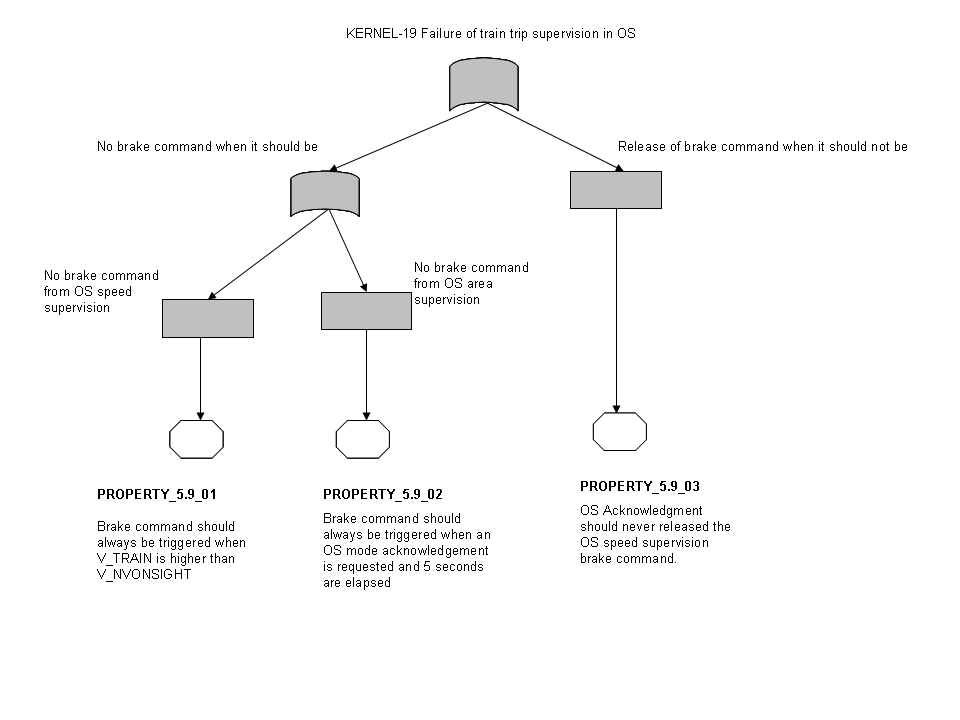
\includegraphics[scale=0.65]{images/kernel19.png}}  
\caption{FTA of Kernel 19}  
\label{fig:FTA_of_kernel_19}
\end{figure}

\chapter{Methodology of the benchmarking and role of WP7}

WP2 is in charge of the definition of the benchmark (this document).

WP7 is in charge of the realisation of the benchmark. The evaluation matrix will be created by WP7, based on the deliverables of WP2. 

The evaluation shall be done by independant persons from those who has done the modelisation and from the provider of the means or tools.

\nocite{*}

\bibliographystyle{unsrt}
\bibliography{erdc}

\appendix

\chapter{ERTMS/ETCS Language}

The purpose of this appendix is to propose common variables / packets / messages for the models.

\emph{ Variables shall be used to encode single data values. Variables cannot be split in minor units. The whole variable has one type (meaning)}
\newline
\emph{Packets are multiple variables grouped into a single unit, with a defined internal structure.}
\newline
\emph{A message (Euroradio/Euroloop) or telegram (Eurobalise) shall be composed of one Header, when needed, a predefined set of variables (only for Radio), when needed, a predefined set of Packets (only for Radio), optional Packets as needed by application.}

All the variables are not defined since it could depend on modelisation choices (especially internal variables of the OBU which are not defined in the SUBSET-026). It is also mainly focussed on chapter 7 and 8 of SUBSET-026.

The following lists are surely not complete but it is a good basis.

\section{\S3.5.3 Establishing a communication session}
\begin{description}
\item [Packet Train to Track :] SUBSET-026 \S7.4.3.3 Packet number 3	Onboard telephone numbers
\item [Message Train to Track :] SUBSET-026 \S8.6.13 Message 155 Initiation of a communication session
\item [Message Train to Track :] SUBSET-026 \S8.6.14 Message 155 Termination of a communication session
\item [Message Train to Track :] SUBSET-026 \S8.6.17	Message 159 Session established
\item [Packet Track to Train :] SUBSET-026 \S7.4.2.1  Packet number 2	System Version order
\item [Packet Track to Train :] SUBSET-026 \S7.4.2.10 Packet number 42	Session Management
\item [Packet Track to Train :] SUBSET-026 \S7.4.2.11.1 Packet number 45	Radio Network registration
\item [Packet Track to Train :] SUBSET-026 \S7.4.2.27 Packet number 131	RBC transition order
\item [Packet Track to Train :] SUBSET-026 \S7.4.2.37.1 Packet number 143	Session Management with neighbouring Radio Infill Unit
\item [Message Track to Train :] SUBSET-026 \S8.7.12	Message 32 RBC/RIU System Version
\item [Message Track to Train :] SUBSET-026 \S8.7.16	Message 38 Initiation of a communication session
\item [Message Track to Train :] SUBSET-026 \S8.7.17	Message 39 Acknowledgement of termination of a communication session
\end{description}

\section{\S5.9 Procedure On-Sight}
\begin{description}
\item [Variable :] SUBSET-026 \S7.5.1.72 M\_MODE
\item [Variable :] SUBSET-026 \S7.5.1.65 M\_LEVEL
\item [Variable :] SUBSET-026 \S7.5.1.162	V\_NVONSIGHT
\item [Variable :] SUBSET-026 \S7.5.1.172	V\_TRAIN
\item [Message Train to Track :] SUBSET-026 \S8.6.7 Message 146 Acknowledgement
\item [Message Train to Track :] SUBSET-026 \S8.6.9 Message 149 Track ahead free granted
\item [Packet Track to Train :] SUBSET-026 \S7.4.2.26 Packet number 80 Mode profile
\item [Packet Track to Train :] SUBSET-026 \S7.4.2.26.2 Packet number 90 Track Ahead Free up to level 2/3 transition location
\item [Message Track to Train :] SUBSET-026 \S8.7.14 Message 34 Track Ahead Free request
\end{description}

\section{\S3.13 Braking curves}
\begin{description}
\item [Variable :] SUBSET-026 \S7.5.0.1 A\_NVMAXREDADH1
\item [Variable :] SUBSET-026 \S7.5.0.2 A\_NVMAXREDADH2
\item [Variable :] SUBSET-026 \S7.5.0.3 A\_NVMAXREDADH3
\item [Variable :] SUBSET-026 \S7.5.0.4 A\_NVP12
\item [Variable :] SUBSET-026 \S7.5.0.5 A\_NVP23
\item [Variable :] SUBSET-026 \S7.5.1.1	D\_ADHESION
\item [Variable :] SUBSET-026 \S7.5.1.4 D\_DP
\item [Variable :] SUBSET-026 \S7.5.1.13	D\_LRBG
\item [Variable :] SUBSET-026 \S7.5.1.19.1	D\_PBD 
\item [Variable :] SUBSET-026 \S7.5.1.19.2	D\_PBDSR 
\item [Variable :] SUBSET-026 \S7.5.1.37	G\_A 
\item [Variable :] SUBSET-026 \S7.5.1.37.1	G\_PBDSR 
\item [Variable :] SUBSET-026 \S7.5.1.38	G\_TSR 
\item [Variable :] SUBSET-026 \S7.5.1.48.1 L\_NVKRINT
\item [Variable :] SUBSET-026 \S7.5.1.49.1	L\_PBDSR
\item [Variable :] SUBSET-026 \S7.5.1.56 L\_TRAIN
\item [Variable :] SUBSET-026 \S7.5.1.57 L\_TRAININT
\item [Variable :] SUBSET-026 \S7.5.1.65 M\_LEVEL
\item [Variable :] SUBSET-026 \S7.5.1.73.1	M\_NVAVADH 
\item [Variable :] SUBSET-026 \S7.5.1.75.1 M\_NVEBCL
\item [Variable :] SUBSET-026 \S7.5.1.75.2 M\_NVKRINT
\item [Variable :] SUBSET-026 \S7.5.1.75.3 M\_NVKTINT
\item [Variable :] SUBSET-026 \S7.5.1.75.4 M\_NVKVINT
\item [Variable :] SUBSET-026 \S7.5.1.110	Q\_GDIR 
\item [Variable :] SUBSET-026 \S7.5.1.115 Q\_LOCACC
\item [Variable :] SUBSET-026 \S7.5.1.123.2 Q\_NVINHSMICPERM
\item [Variable :] SUBSET-026 \S7.5.1.123.3 Q\_NVKINT
\item [Variable :] SUBSET-026 \S7.5.1.123.4 Q\_NVKVINTSET
\item [Variable :] SUBSET-026 \S7.5.1.126.1	Q\_PBDSR
\item [Variable :] SUBSET-026 \S7.5.1.155	V\_AXLELOAD 
\item [Variable :] SUBSET-026 \S7.5.1.156	V\_DIFF 
\item [Variable :] SUBSET-026 \S7.5.1.157	V\_LOA 
\item [Variable :] SUBSET-026 \S7.5.1.157.1	V\_LX 
\item [Variable :] SUBSET-026 \S7.5.1.158	V\_MAIN 
\item [Variable :] SUBSET-026 \S7.5.1.159	V\_MAMODE 
\item [Variable :] SUBSET-026 \S7.5.1.160	V\_MAXTRAIN 
\item [Variable :] SUBSET-026 \S7.5.1.161	V\_NVALLOWOVTRP 
\item [Variable :] SUBSET-026 \S7.5.1.161.1	V\_NVKVINT 
\item [Variable :] SUBSET-026 \S7.5.1.161.2	V\_NVLIMSUPERV 
\item [Variable :] SUBSET-026 \S7.5.1.162	V\_NVONSIGHT 
\item [Variable :] SUBSET-026 \S7.5.1.163	V\_NVSUPOVTRP
\item [Variable :] SUBSET-026 \S7.5.1.164	V\_NVREL 
\item [Variable :] SUBSET-026 \S7.5.1.165	V\_NVSHUNT 
\item [Variable :] SUBSET-026 \S7.5.1.166	V\_NVSTFF 
\item [Variable :] SUBSET-026 \S7.5.1.167	V\_NVUNFIT
\item [Variable :] SUBSET-026 \S7.5.1.168	V\_RELEASEDP 
\item [Variable :] SUBSET-026 \S7.5.1.169	V\_RELEASEOL 
\item [Variable :] SUBSET-026 \S7.5.1.170	V\_REVERSE
\item [Variable :] SUBSET-026 \S7.5.1.171	V\_STATIC 
\item [Variable :] SUBSET-026 \S7.5.1.172	V\_TRAIN
\item [Variable :] SUBSET-026 \S7.5.1.173	V\_TSR 
\item [Packet Track to Train :] SUBSET-026 \S7.4.2.6 Packet number 21 Gradient Profile
\item [Packet Track to Train :] SUBSET-026 \S7.4.2.37 Packet number 141	Default Gradient for Temporary Speed Restriction
\end{description}

\section{\S4.6.2 and 4.6.3 Transition table}
\begin{description}
\item [Variable :] SUBSET-026 \S7.5.1.13 D\_LRBG
\item [Variable :] SUBSET-026 \S7.5.1.72 M\_MODE
\item [Variable :] SUBSET-026 \S7.5.1.65 M\_LEVEL
\item [Variable :] SUBSET-026 \S7.5.1.172	V\_TRAIN
\item [Message Train to Track :] SUBSET-026 \S8.6.2 Message 130 Request for Shunting
\item [Message Train to Track :] SUBSET-026 \S8.6.7 Message 146 Acknowledgement
\item [Packet Track to Train :] SUBSET-026 \S7.4.2.3 Packet number 12 Level 1 Movement Authority
\item [Packet Track to Train :] SUBSET-026 \S7.4.2.4 Packet number 15 Level 2/3 Movement Authority
\item [Packet Track to Train :] SUBSET-026 \S7.4.2.6 Packet number 21 Gradient Profile
\item [Packet Track to Train :] SUBSET-026 \S7.4.2.7 Packet number 27 International Static Speed Profile
\item [Packet Track to Train :] SUBSET-026 \S7.4.2.37 Packet number 141	Default Gradient for Temporary Speed Restriction
\item [Packet Track to Train :] SUBSET-026 \S7.4.2.26 Packet number 80 Mode profile 
\item [Message Track to Train :] SUBSET-026 \S8.7.2 Message 3 Movement Authority
\item [Message Track to Train :] SUBSET-026 \S8.7.10 Message 27 SH Refused
\item [Message Track to Train :] SUBSET-026 \S8.7.11 Message 28 SH Authorised
\end{description}

\section{\S4.8.3.2 From National System X}
\begin{description}
\item [Variable :] SUBSET-026 \S7.5.1.65 M\_LEVEL
\item [Packet Track to Train :] SUBSET-026 \S7.4.2.9 Packet Number 41 Level Transition Order
\item [Packet STM to Train :] SUBSET-058 \S7.2.8 Packet STM-16 Transition variables STM max speed from STM 
\item [Packet STM to Train) :] SUBSET-058 \S7.2.9 Packet STM-17 Transition variables STM system speed and distance from STM 
\end{description}

\section{\S3.6.3.2 Location, Continuous Profile Data and Non-Continuous Profile Data}
\begin{description}
\item [Variable :] SUBSET-026 \S7.5.1.13 D\_LRBG
\item [Variable :] SUBSET-026 \S7.5.1.22 D\_REF
\item [Variable :] SUBSET-026 \S7.5.1.90 NID\_LRBG
\item [Variable :] SUBSET-026 \S7.5.1.94 NID\_PRVLRBG
\item [Variable :] SUBSET-026 \S7.5.1.103 Q\_DIR
\item [Variable :] SUBSET-026 \S7.5.1.104 Q\_DIRLRBG
\item [Variable :] SUBSET-026 \S7.5.1.105 Q\_DIRTRAIN
\item [Variable :] SUBSET-026 \S7.5.1.106 Q\_DLRBG
\item [Packet Track to Train :] SUBSET-026 \S7.4.2.5 Packet number 16	Repositioning Information
\item [Message Track to Train :] SUBSET-026 \S8.7.13 Message 33 MA with Shifted Location Reference
\end{description}

\section{\S3.8.3 Structure of Movement Authority and §3.8.5 Update of Movement Authority}
\begin{description}
\item [Packet Track to Train :] SUBSET-026 \S7.4.2.3 Packet number 12 Level 1 Movement Authority
\item [Packet Track to Train :] SUBSET-026 \S7.4.2.4 Packet number 15 Level 2/3 Movement Authority 
\item [Packet Track to Train :] SUBSET-026 \S7.4.2.32 Packet number 136 Infill location reference
\item [Message Track to Train :] SUBSET-026 \S8.7.2 Message 3 Movement Authority
\item [Message Track to Train :] SUBSET-026 \S8.7.13 Message 33 MA with Shifted Location Reference
\item [Message Track to Train :] SUBSET-026 \S8.7.15 Message 37 Infill MA
\end{description}

\section{\S3.11.3 Static Speed Profile and §3.11.12 Gradients}
\begin{description}
\item [Packet Track to Train :] SUBSET-026 \S7.4.2.6 Packet number 21 Gradient Profile
\item [Packet Track to Train :] SUBSET-026 \S7.4.2.7 Packet number 27 International Static Speed Profile
\item [Packet Track to Train :] SUBSET-026 \S7.4.2.37 Packet number 141	Default Gradient for Temporary Speed Restriction
\end{description}

\section{\S8.7.2 Movement Authority message}
\begin{description}
\item [Packet Track to Train :] SUBSET-026 \S7.4.2.4 Packet number 15 Level 2/3 Movement Authority
\item [Message Track to Train :] SUBSET-026 \S8.7.2 Message 3 Movement Authority 
\end{description}

\end{document}
Local Variables:
ispell-local-dictionary: "english"
End:

% LocalWords:  SRS ERTMS ETCS UNISIG
*)
